\documentclass{article}%
\usepackage[T1]{fontenc}%
\usepackage[utf8]{inputenc}%
\usepackage{lmodern}%
\usepackage{textcomp}%
\usepackage{lastpage}%
\usepackage{authblk}%
\usepackage{graphicx}%
%
\title{An Extracellular Subtilase Switch for Immune Priming in Arabidopsis}%
\author{Mary Simmons}%
\affil{Department of Oral and Maxillofacial Surgery, Hyogo College of Medicine, Nishinomiya, Hyogo 663{-}8501, Japan, Department of Genetics, Hyogo College of Medicine, Nishinomiya, Hyogo 663{-}8501, Japan}%
\date{01{-}01{-}2012}%
%
\begin{document}%
\normalsize%
\maketitle%
\section{Abstract}%
\label{sec:Abstract}%
By Dr. Anthony Alix\newline%
Cellular antenna failure is probably one of the most common causes of cancer, and poses tremendous challenges in future applications of biologic antennae, including commercial satellites.\newline%
Recent advances in Ku{-}band satellite technology has greatly increased the ubiquity of satellite communication. A range of high frequency spectroscopic methods and fusion of biologics gases has developed to enable direct coupling of the radio signal with the CO2 emitted by the gas. The resulting signal is easily beamed into a cell and swiftly transmitted to a antenna.\newline%
Defensive antennae in birds, satellites, and vehicles transmit signals at a range of 8 to 15 MHz and provide range of more than 100 feet. For some cellular telephones, antennas can be moved around, creating an endless network of cell tower structures, and 6D antennas can serve as the foundation of a cellular network. In complete grid structure mode, there is no movement, transmission distance, or base stations, creating a network of redundant tower structures that can be manipulated on the fly to act as carrier gates or gateways. These centralized towers or complexes can be constructed in less than a year, an elaborate process of building new additions and retrofitting antennas.\newline%
The barriers of cellular proliferation are both real and present. With an increasing flood of new applications for cellular antennae in the marketplace, radiation exposure has to be monitored, in much the same way as environmental factors are monitored.\newline%
The radiation risks are represented as various doses of radiation, from several hundred to hundreds of millirems per year per patient. Any overflight of a geostationary orbit or across an international boundary, if ingested, is sufficient to cause substantial harm. A number of countries set stringent safety requirements for cell{-}based use.\newline%
The results of a large, ongoing international study showed that cancer incidence in American women in 1990 was 6.6 percent, with breast cancer, which became the largest cause of death for American women, dying 7.6 percent short of a rate of prostate cancer. Comparatively, compared to the 20 percent rate of breast cancer and a 10 percent rate of prostate cancer in the US today, it is unknown whether the proportion of breast cancer, prostate cancer, and overall mortality from breast cancer has changed since 1990.\newline%
The carcinogenic effect of radiation is important, and some very controversial, issues involving cellular technology can arise. They include:\newline%
1. Will our environment and our children be vulnerable to harmful radiation in the future?\newline%
2. How much should the public be informed about the real dangers associated with cellular radiation?\newline%
3. How confident are the scientists involved in these studies? Do they have adequate funding, or will they be scared away from their research if they do not receive funding?

%
\subsection{Image Analysis}%
\label{subsec:ImageAnalysis}%


\begin{figure}[h!]%
\centering%
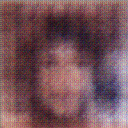
\includegraphics[width=150px]{500_fake_images/samples_5_41.png}%
\caption{A Close Up Of A Person Holding A Pair Of Scissors}%
\end{figure}

%
\end{document}